\section{RTC::Fsm\-Participant\-Action Interface Reference}
\label{interfaceRTC_1_1FsmParticipantAction}\index{RTC::FsmParticipantAction@{RTC::FsmParticipantAction}}
Execution\-Semantics::Fsm\-Participant\-Action interface.  


{\tt import \char`\"{}RTC.idl\char`\"{};}

Inheritance diagram for RTC::Fsm\-Participant\-Action::\begin{figure}[H]
\begin{center}
\leavevmode
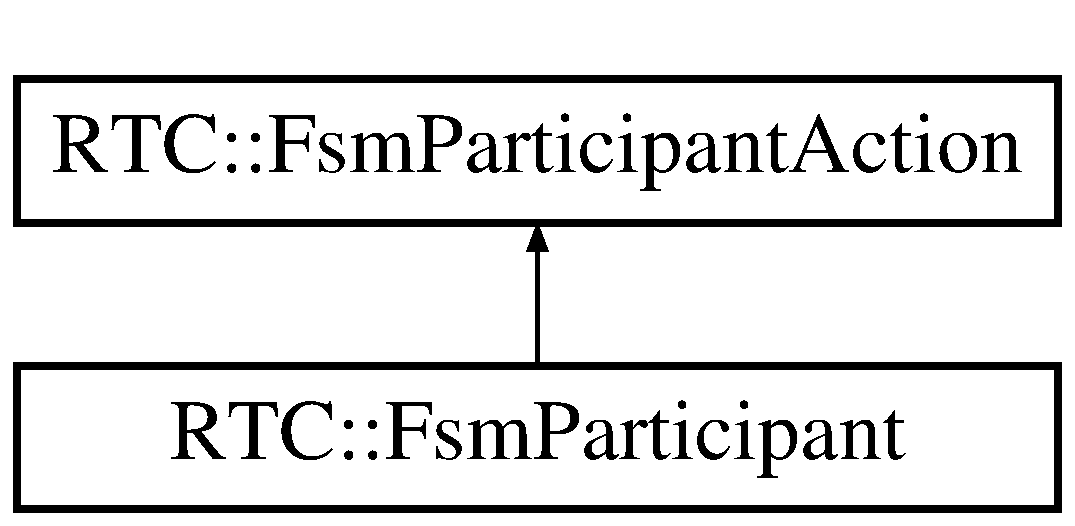
\includegraphics[height=2cm]{interfaceRTC_1_1FsmParticipantAction}
\end{center}
\end{figure}
\subsection*{Public Member Functions}
\begin{CompactItemize}
\item 
{\bf Return\-Code\_\-t} {\bf on\_\-action} (in {\bf Unique\-Id} ec\_\-id)
\end{CompactItemize}


\subsection{Detailed Description}
Execution\-Semantics::Fsm\-Participant\-Action interface. 



\subsection{Member Function Documentation}
\index{RTC::FsmParticipantAction@{RTC::Fsm\-Participant\-Action}!on_action@{on\_\-action}}
\index{on_action@{on\_\-action}!RTC::FsmParticipantAction@{RTC::Fsm\-Participant\-Action}}
\subsubsection{\setlength{\rightskip}{0pt plus 5cm}{\bf Return\-Code\_\-t} RTC::Fsm\-Participant\-Action::on\_\-action (in {\bf Unique\-Id} {\em ec\_\-id})}\label{interfaceRTC_1_1FsmParticipantAction_RTC_1_1FsmParticipantActiona0}




The documentation for this interface was generated from the following file:\begin{CompactItemize}
\item 
{\bf RTC.idl}\end{CompactItemize}
